\subsection{Attori}
\label{ss:attori}
In questa sezione, per la definizione degli attori abbiamo deciso di riutilizzare le persona definite in \hyperref[s:persona]{3.3 Persona}.
Sebbene le avessimo già dettagliate abbondantemente nel capitolo \hyperref[c:studio-fattibilita]{3 Studio di Fattibilità}, abbiamo ritenuto significativo caratterizzarle anche mediante il \textit{Diagramma C\&A} nei termini delle sei caratteristiche maggiormente impattanti le scelte progettuali: competenza tecnica, di dominio, di linguaggio, abilità fisiche, motivazione e concentrazione.

\noindent
\subsubsection{Attori diretti e indiretti}
\label{sss:attori-diretti-indiretti}
Gli attori cui siamo pervenuti pertanto sono:
\begin{itemize}
    \item Diretti:
    \begin{itemize}
        \item Fruizione:
        \begin{itemize}
            \item Giornalista di una testata nazionale;
            \item Giornalista d'agenzia;
            \item Giornalista di una testata locale;
            \item Cittadino esperto;
            \item Blogger;
        \end{itemize}
    \end{itemize}
    \item Indiretti:
    \begin{itemize}
        \item Amministrazione database e dashboard:
        \begin{itemize}
            \item Amministratore di database;
        \end{itemize}
        \item Fruizione da dispositivo mobile:
        \begin{itemize}
            \item Cittadino che visita la dashboard da un dispositivo mobile.
        \end{itemize}
    \end{itemize}
\end{itemize}

\subsubsection{Diagrammi C\&A}
\label{sss:diagrammi-c_and_a}
Abbiamo caratterizzato ogni attore individuato nei termini delle competenze e abilità che presenta e che impattano in maniera più significativa sulle scelte progettuali, per poi mapparli ciascuno sul Diagramma C\&A, così da avere una visione d'insieme.
Ci siamo concentrati sugli attori diretti, articolando l'analisi tra le persona protagoniste (giornalisti) e le persona secondarie (blogger e cittadino esperto).\\
Il risultato ottenuto si può vedere nei successivi diagrammi:
\begin{figure}[H]
    \centering
    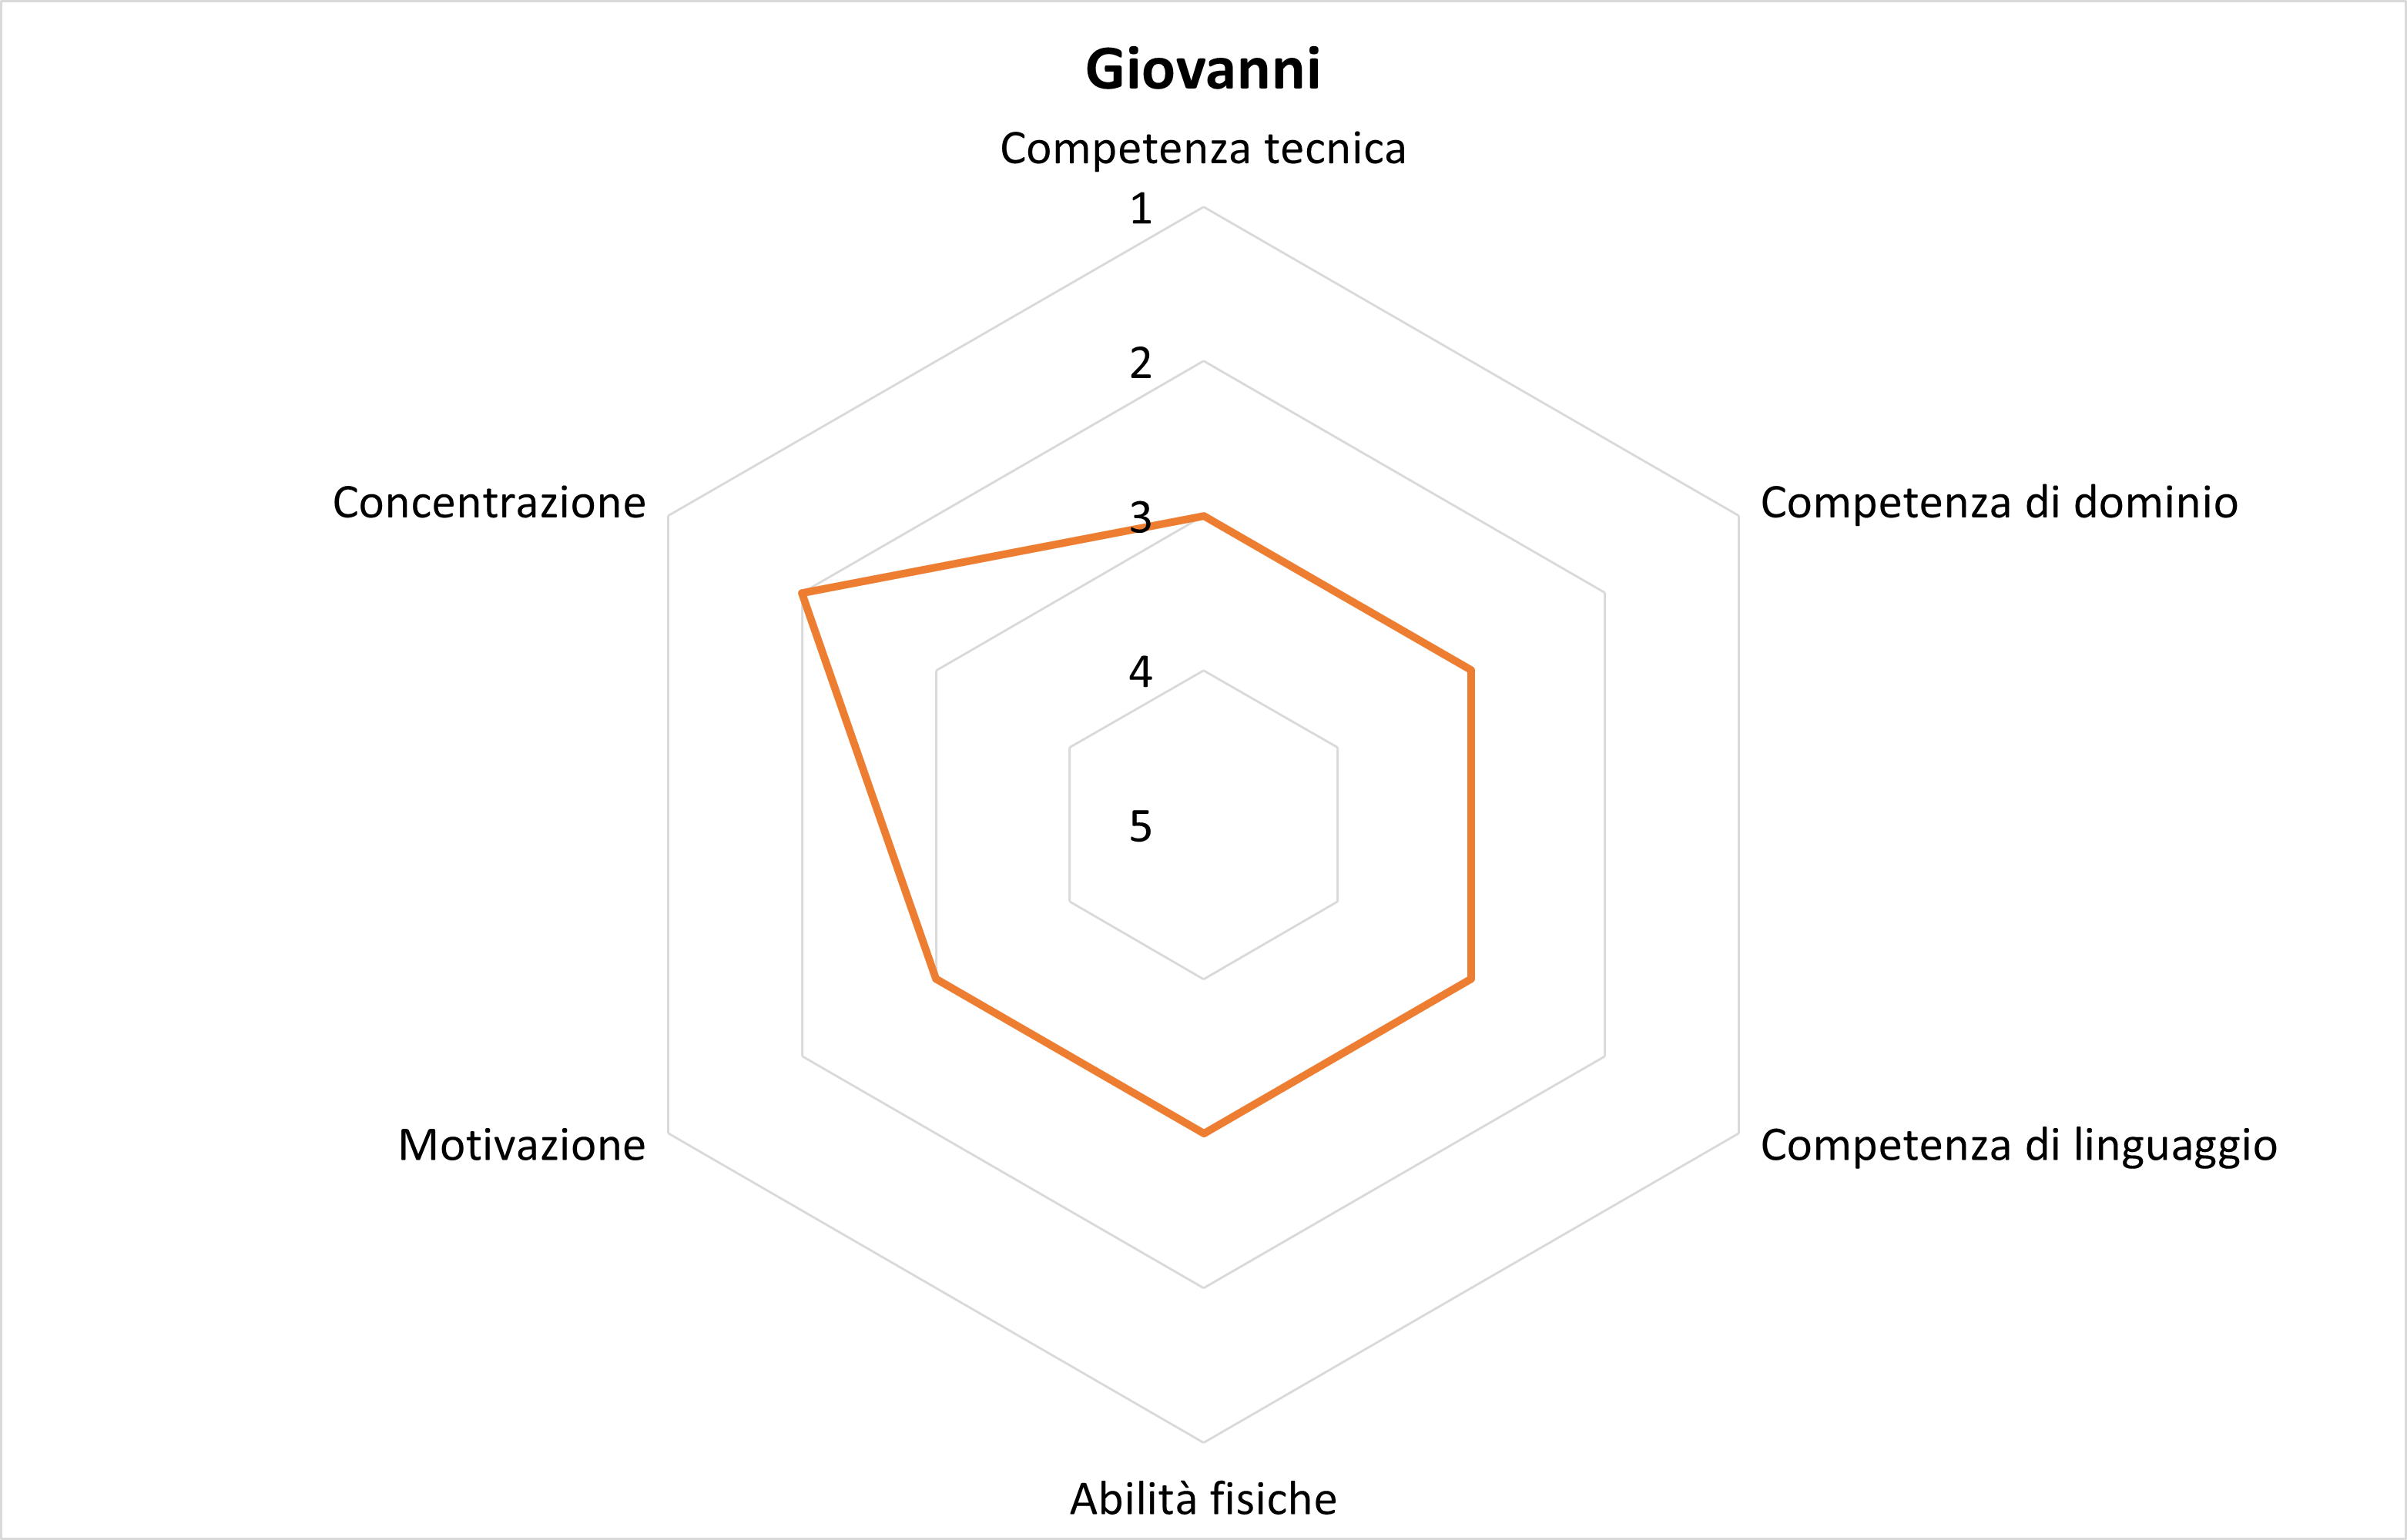
\includegraphics[width=0.5\columnwidth]{assets/images/proposta-design/caos/giovanni}
    \caption{Diagramma C\&A per Giovanni, il giornalista di una testata nazionale.}
\end{figure}

\begin{figure}[H]
    \centering
    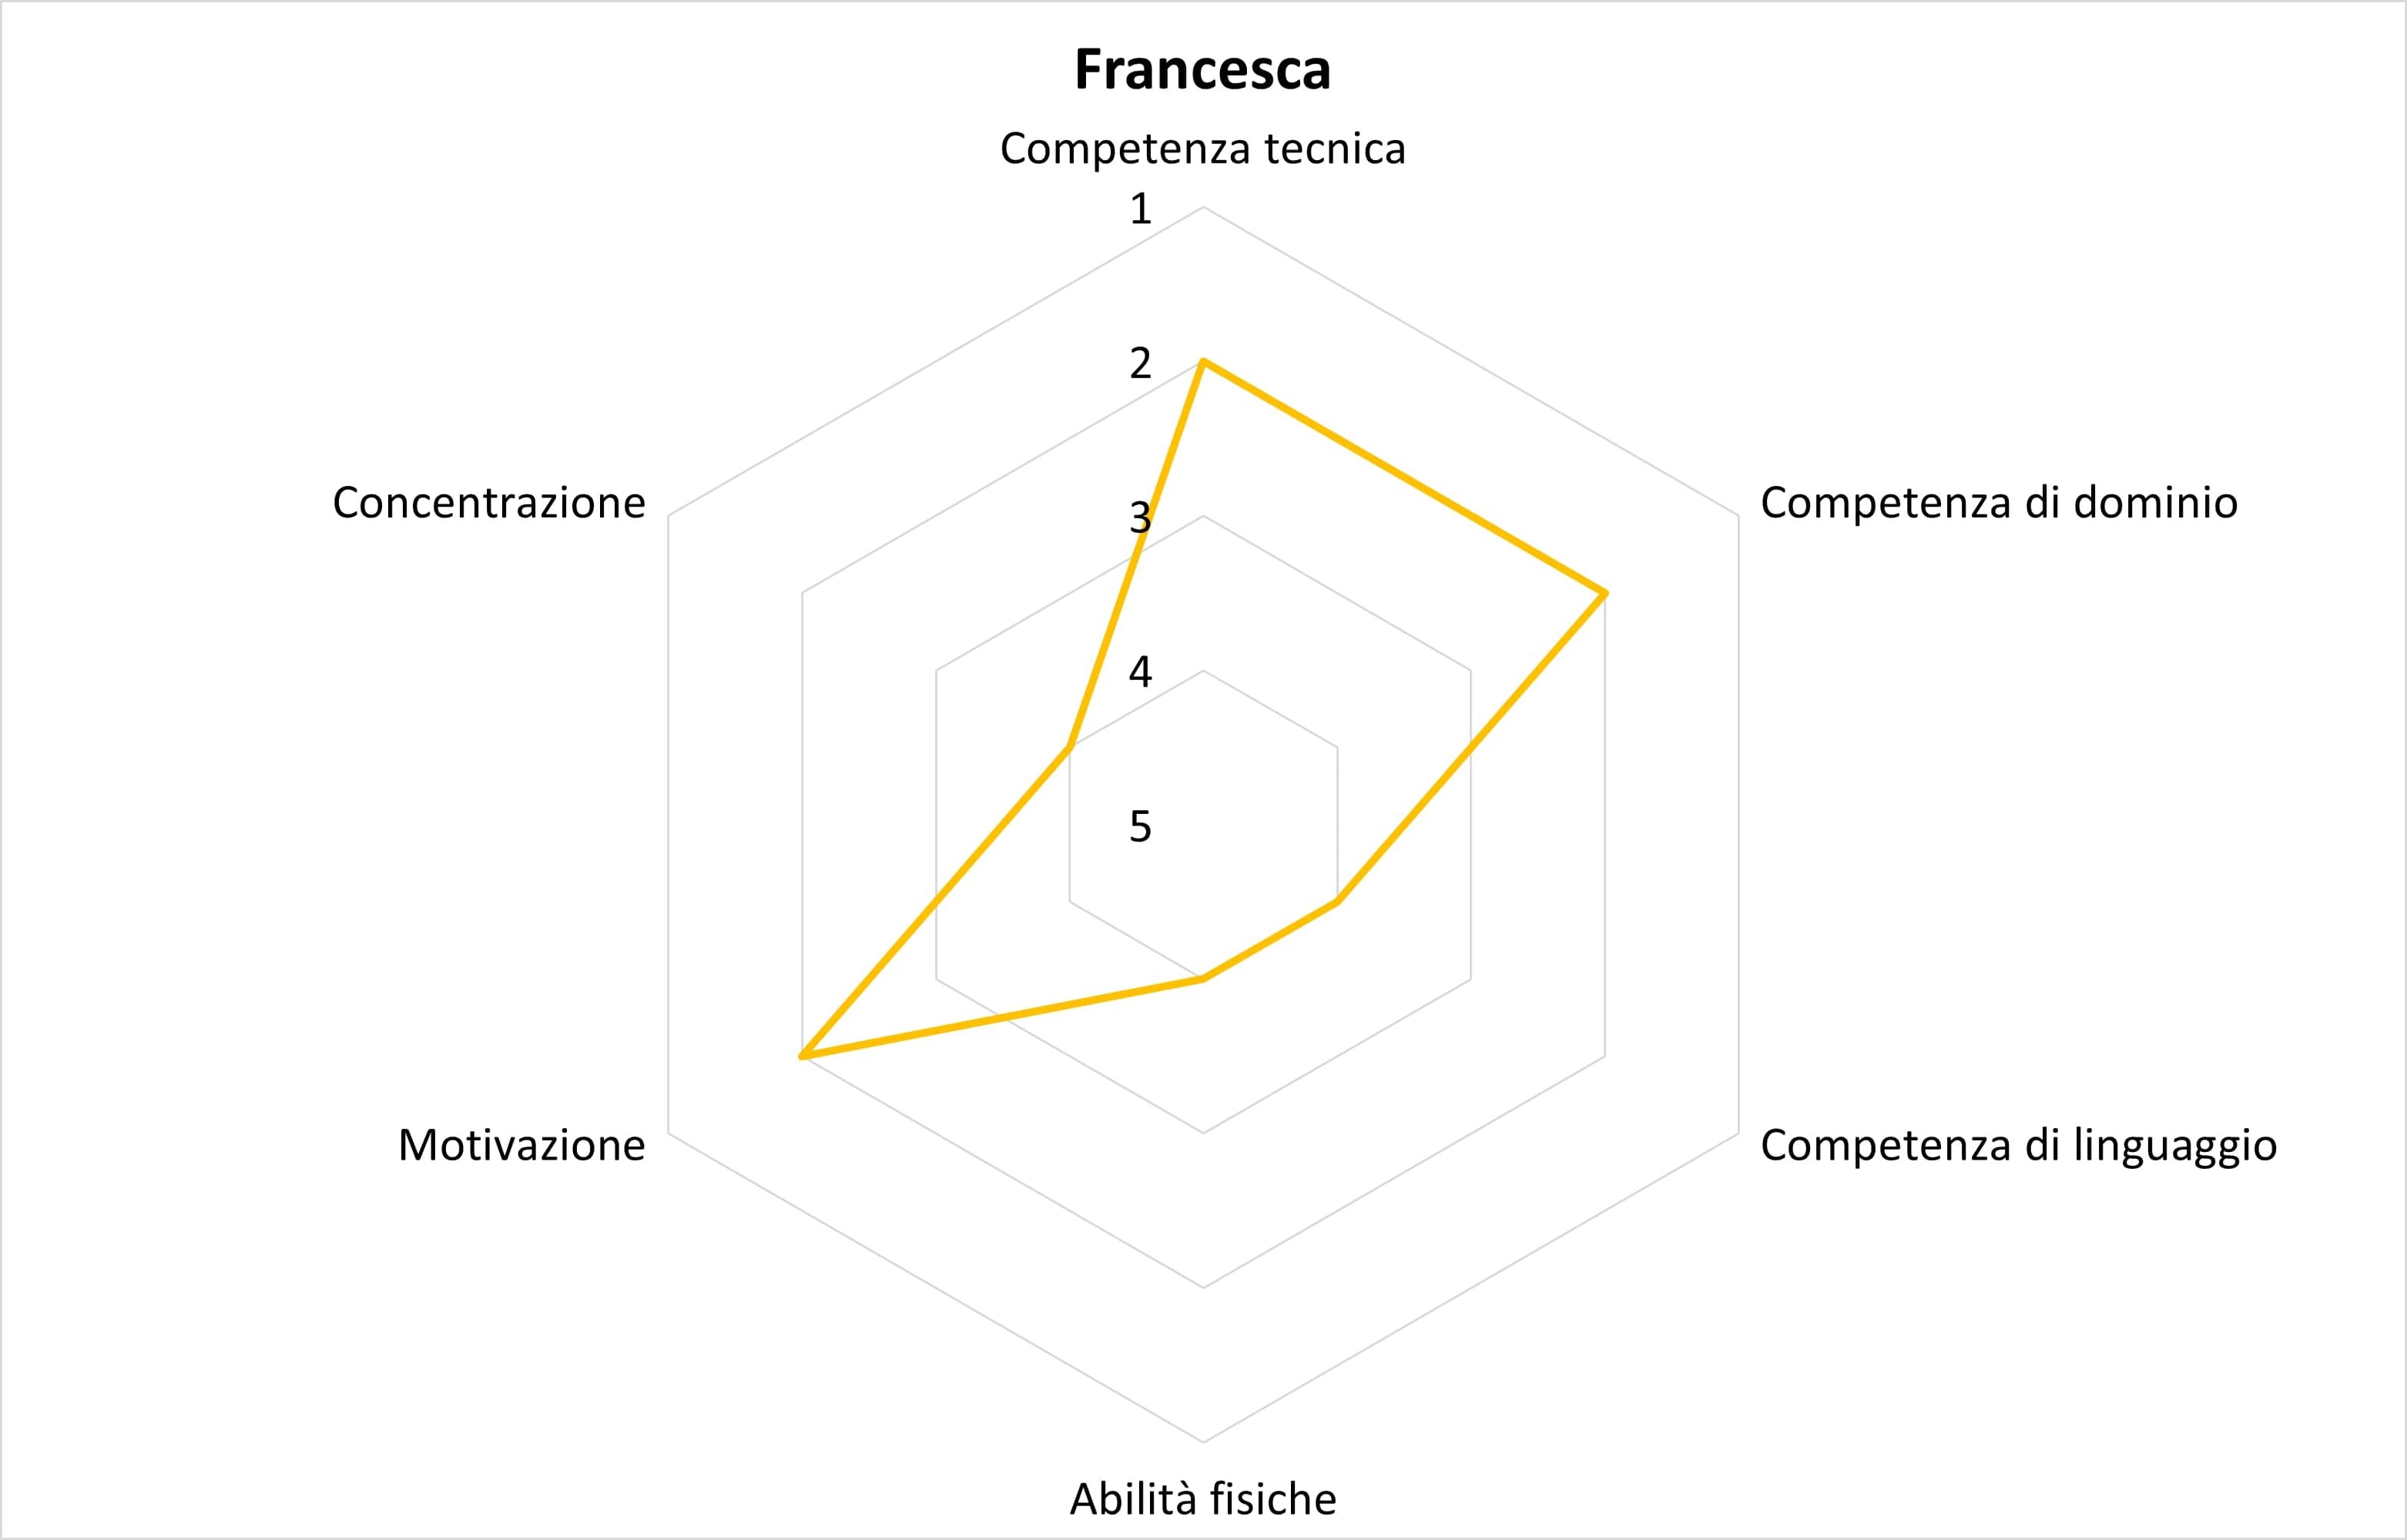
\includegraphics[width=0.5\columnwidth]{assets/images/proposta-design/caos/francesca}
    \caption{Diagramma C\&A per Francesca, la giornalista di una testata locale.}
\end{figure}

\begin{figure}[H]
    \centering
    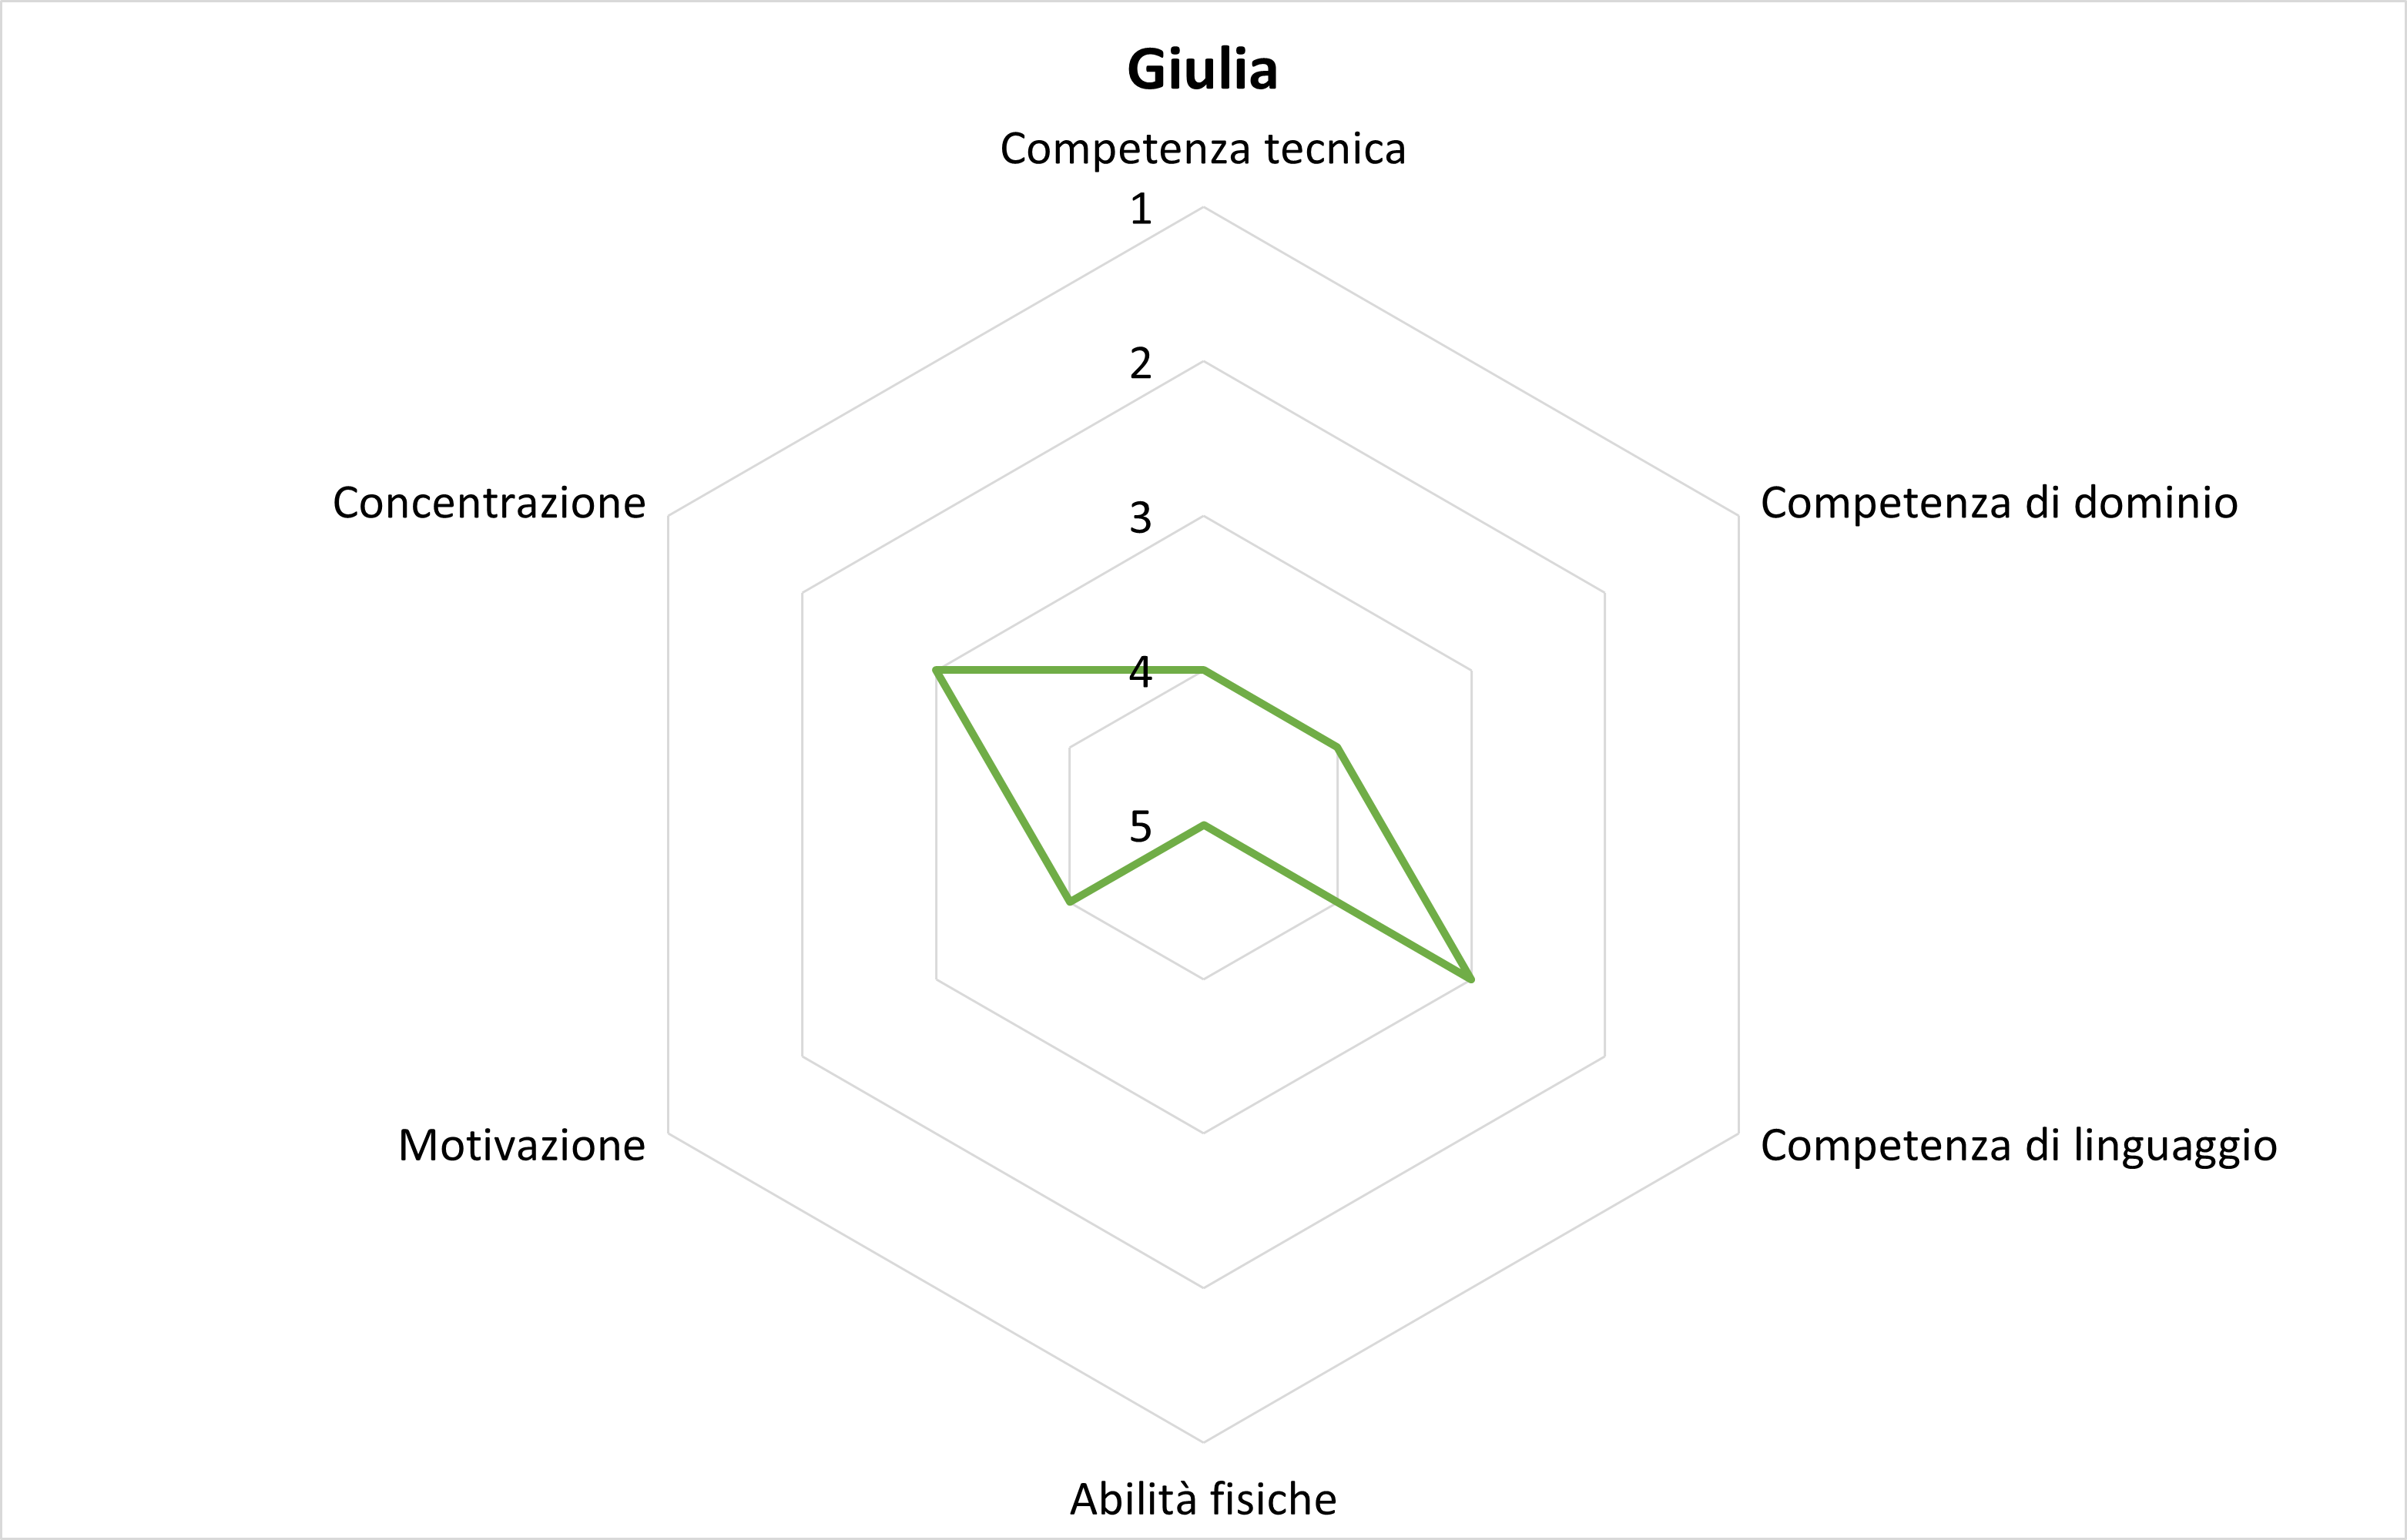
\includegraphics[width=0.5\columnwidth]{assets/images/proposta-design/caos/giulia}
    \caption{Diagramma C\&A per Giulia, la giornalista di una agenzia di stampa.}
\end{figure}

\begin{figure}[H]
    \centering
    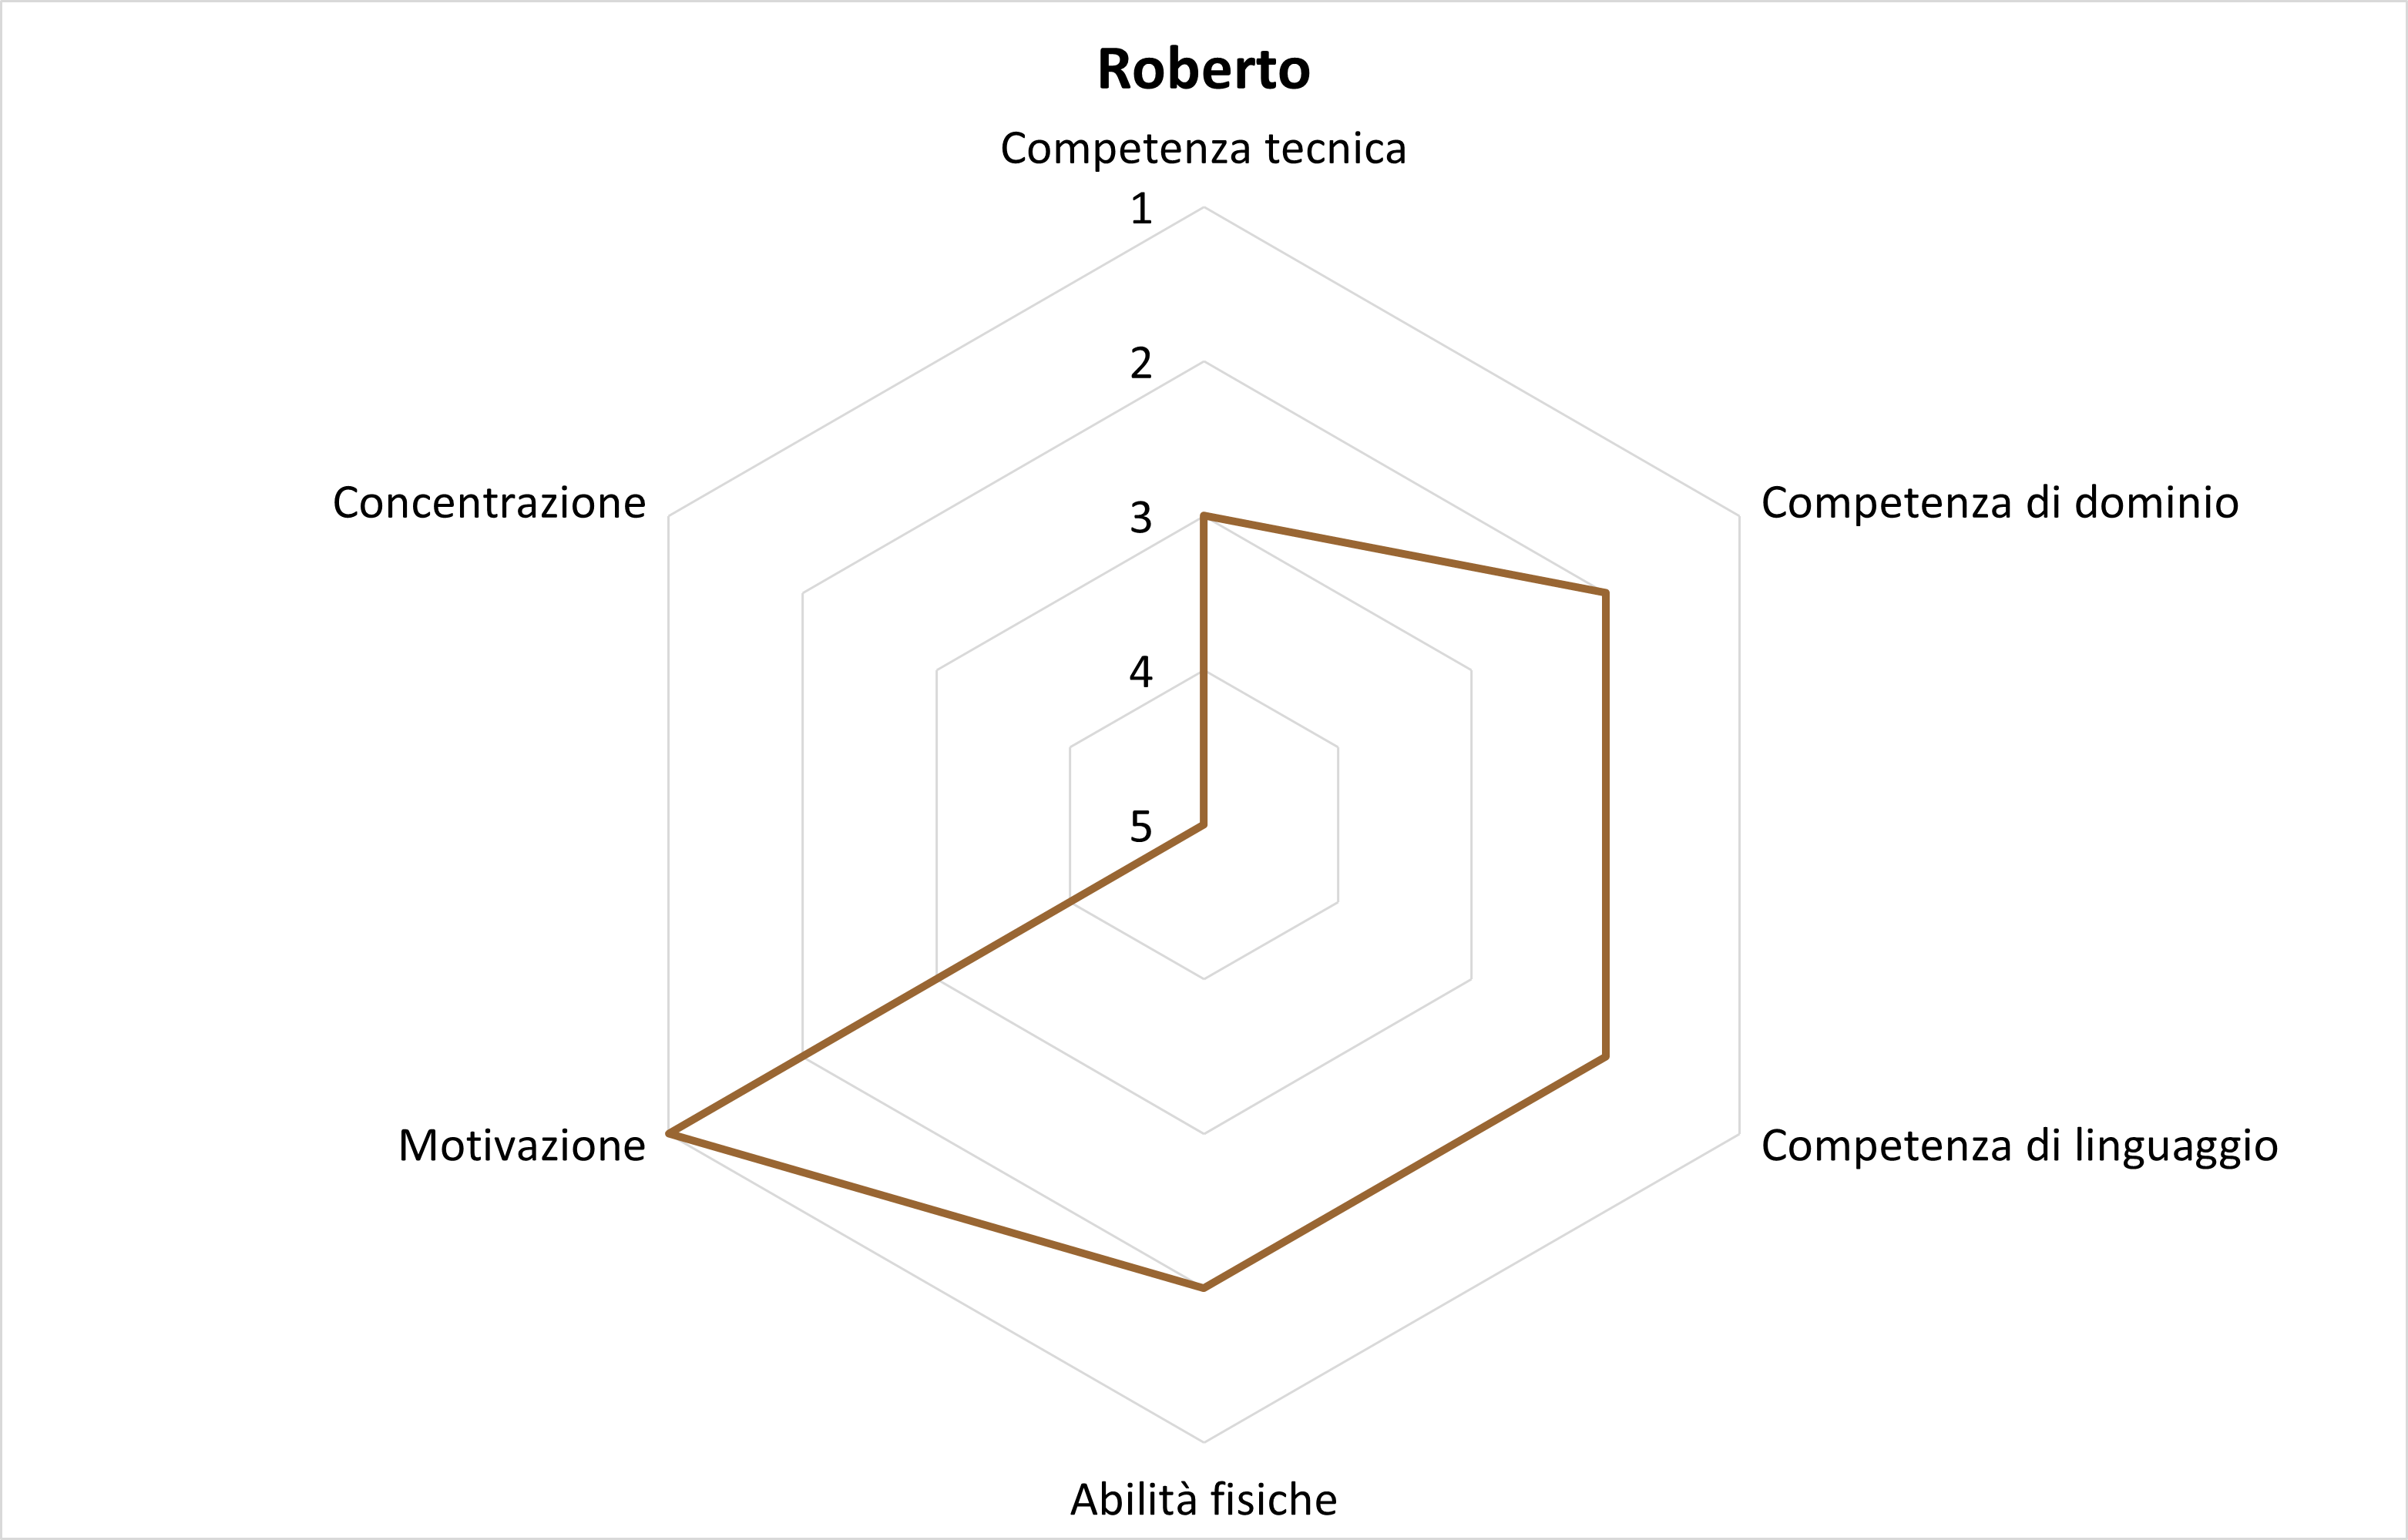
\includegraphics[width=0.5\columnwidth]{assets/images/proposta-design/caos/roberto}
    \caption{Diagramma C\&A per Roberto, il blogger.}
\end{figure}

\begin{figure}[H]
    \centering
    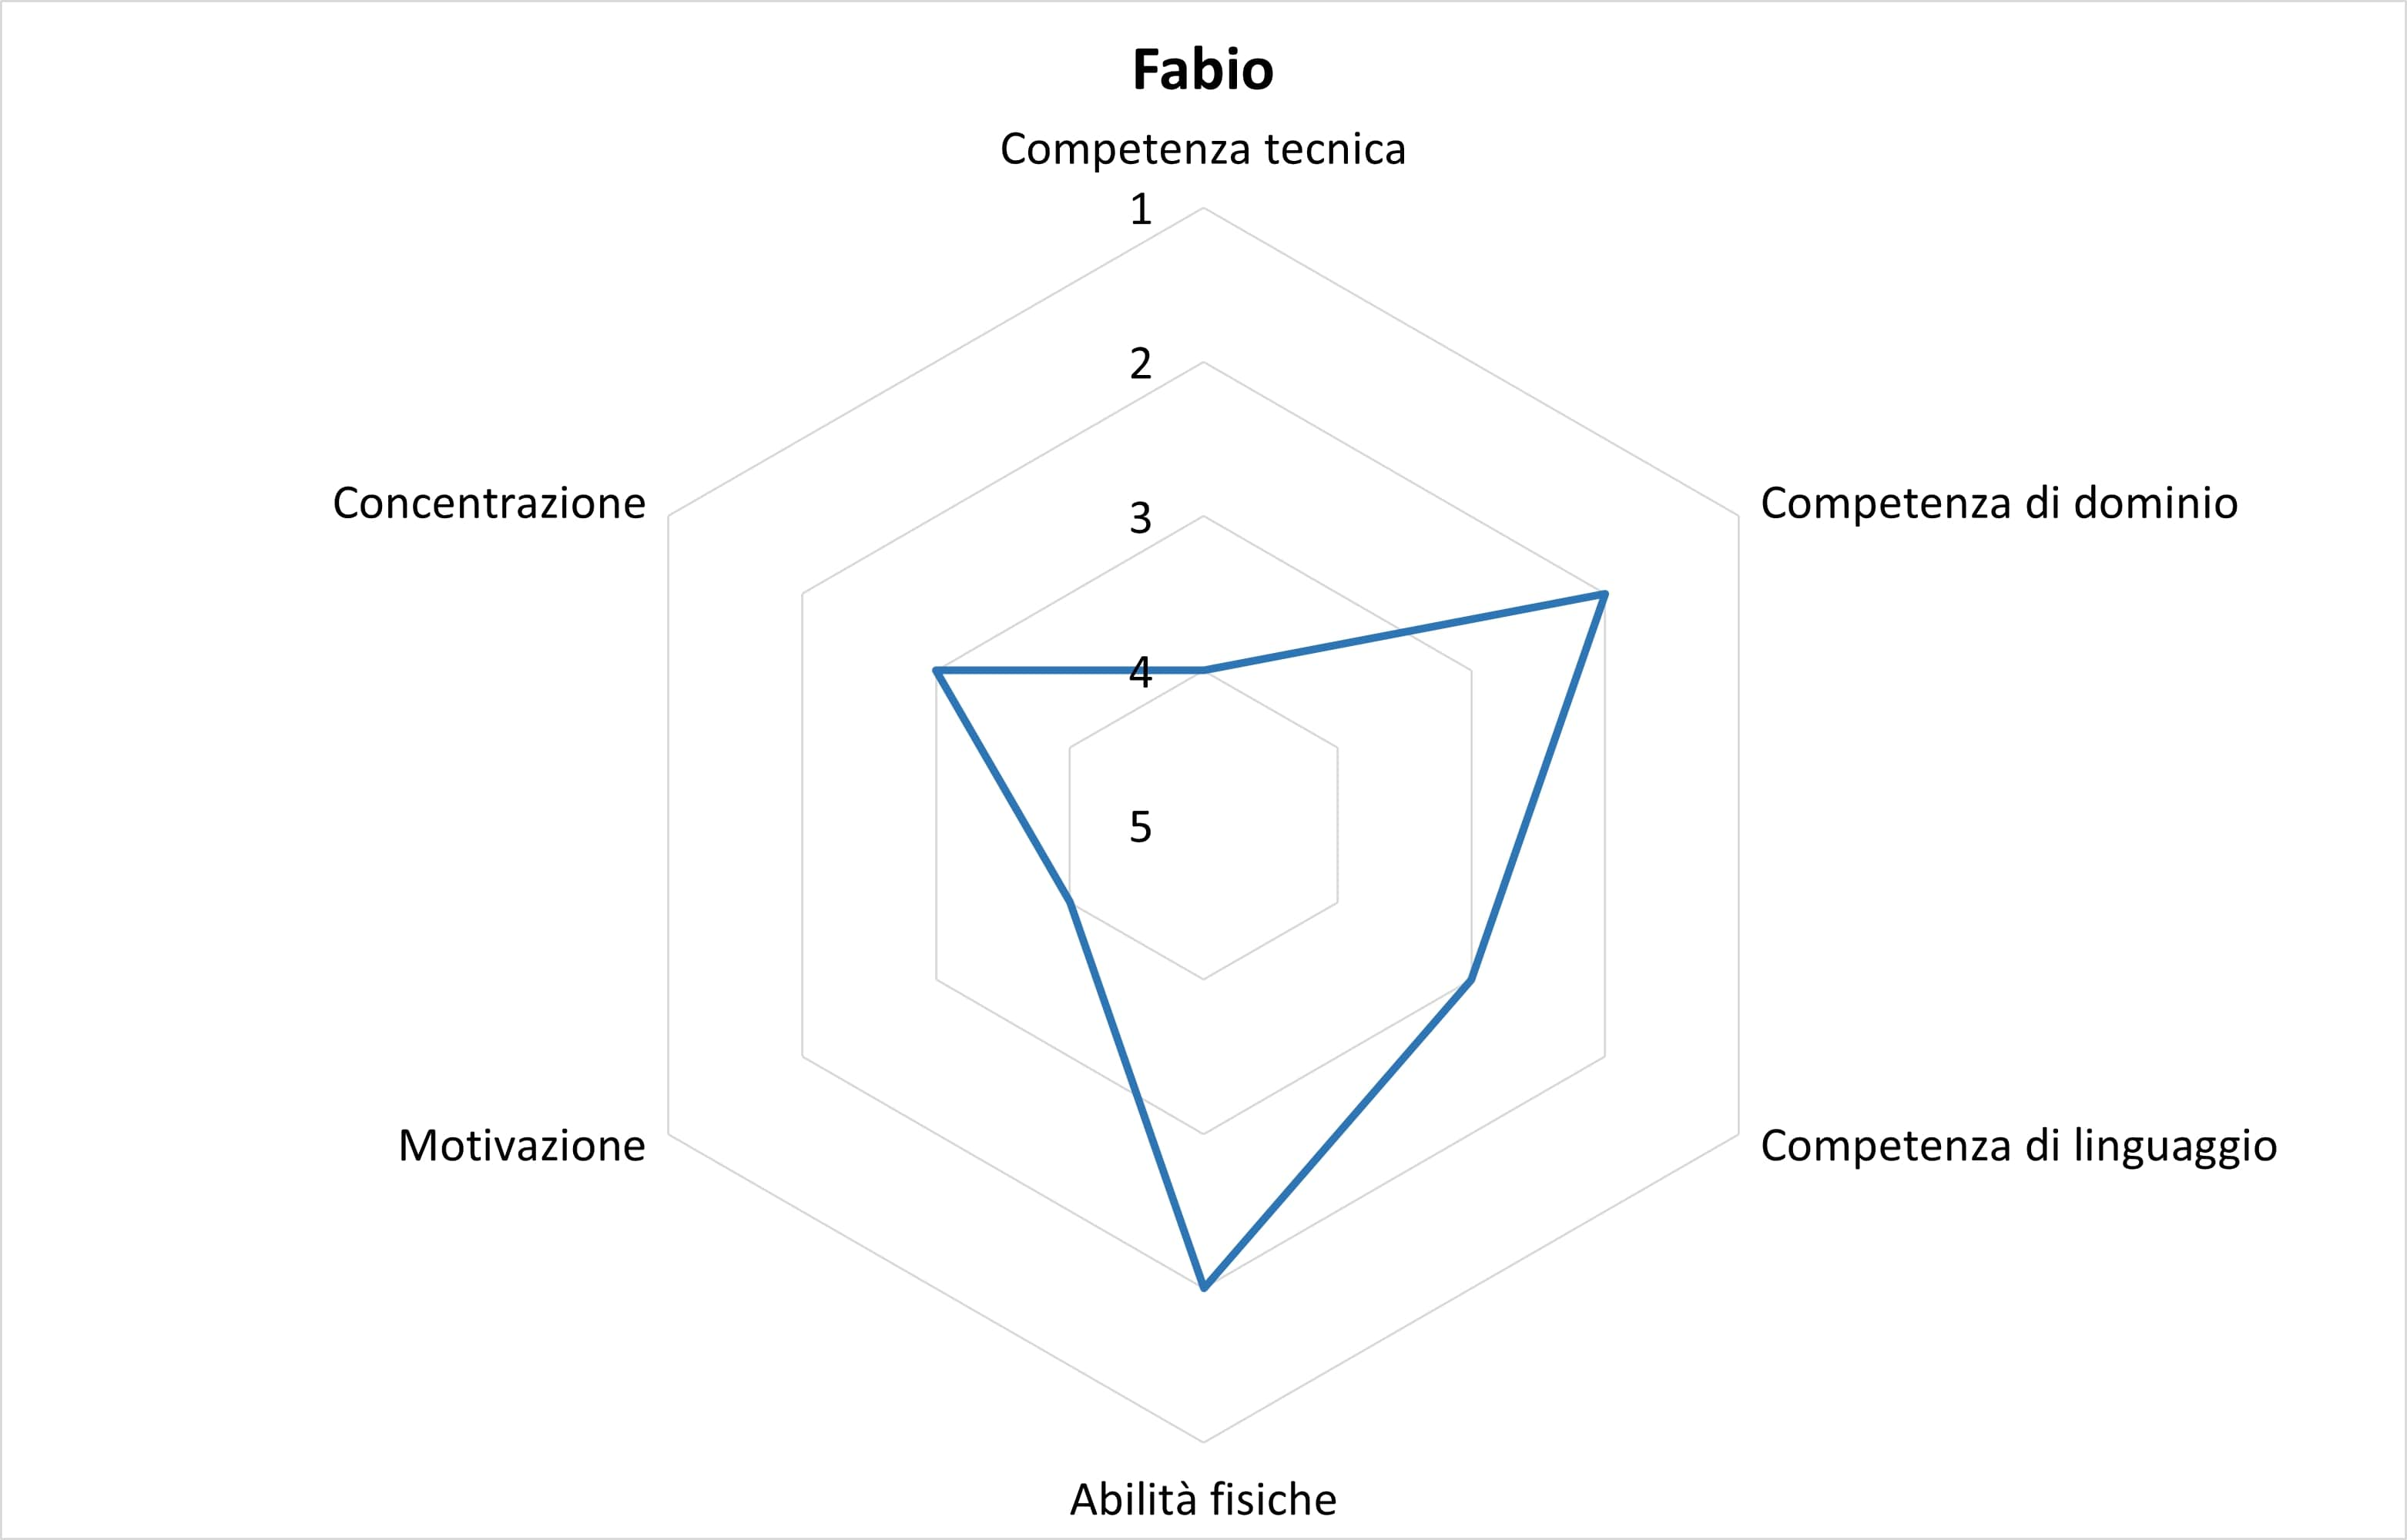
\includegraphics[width=0.5\columnwidth]{assets/images/proposta-design/caos/fabio}
    \caption{Diagramma C\&A per Fabio, il cittadino esperto.}
\end{figure}

\noindent
Riguardo ai giornalisti, sono emerse scarse competenze tecniche e di dominio, il che li rende inclini a errori (\textit{mistake}\footnote{Con il termine \textit{mistake} si intende un'errata comprensione del problema, cui segue un'esecuzione di azioni errate.}), per cui nella nostra riprogettazione della dashboard abbiamo previsto numerose spiegazioni \textit{on-demand}\footnote{Espressione usata con riferimento a beni o servizî che vengono resi disponibili su richiesta del consumatore o dell'utente.} sulle componenti trattanti concetti più complicati.
Inoltre, questi attori presentano scarsa concentrazione a causa dell'ambiente in cui operano, nonché bassa motivazione per via della volontarietà di adozione della dashboard tra varie alternative.
Pertanto, per invogliare gli utenti a consultare la dashboard oggetto della nostra riprogettazione, abbiamo posto l'enfasi sull'autorevolezza dell'istituzione che la gestisce, mentre per facilitare l'interazione anche in contesti con tante distrazioni, abbiamo previsto un'interfaccia chiara, consistente e che non richiede elevati carichi cognitivi, grazie alle sue numerose componenti grafiche.
\begin{figure}[H]
    \centering
    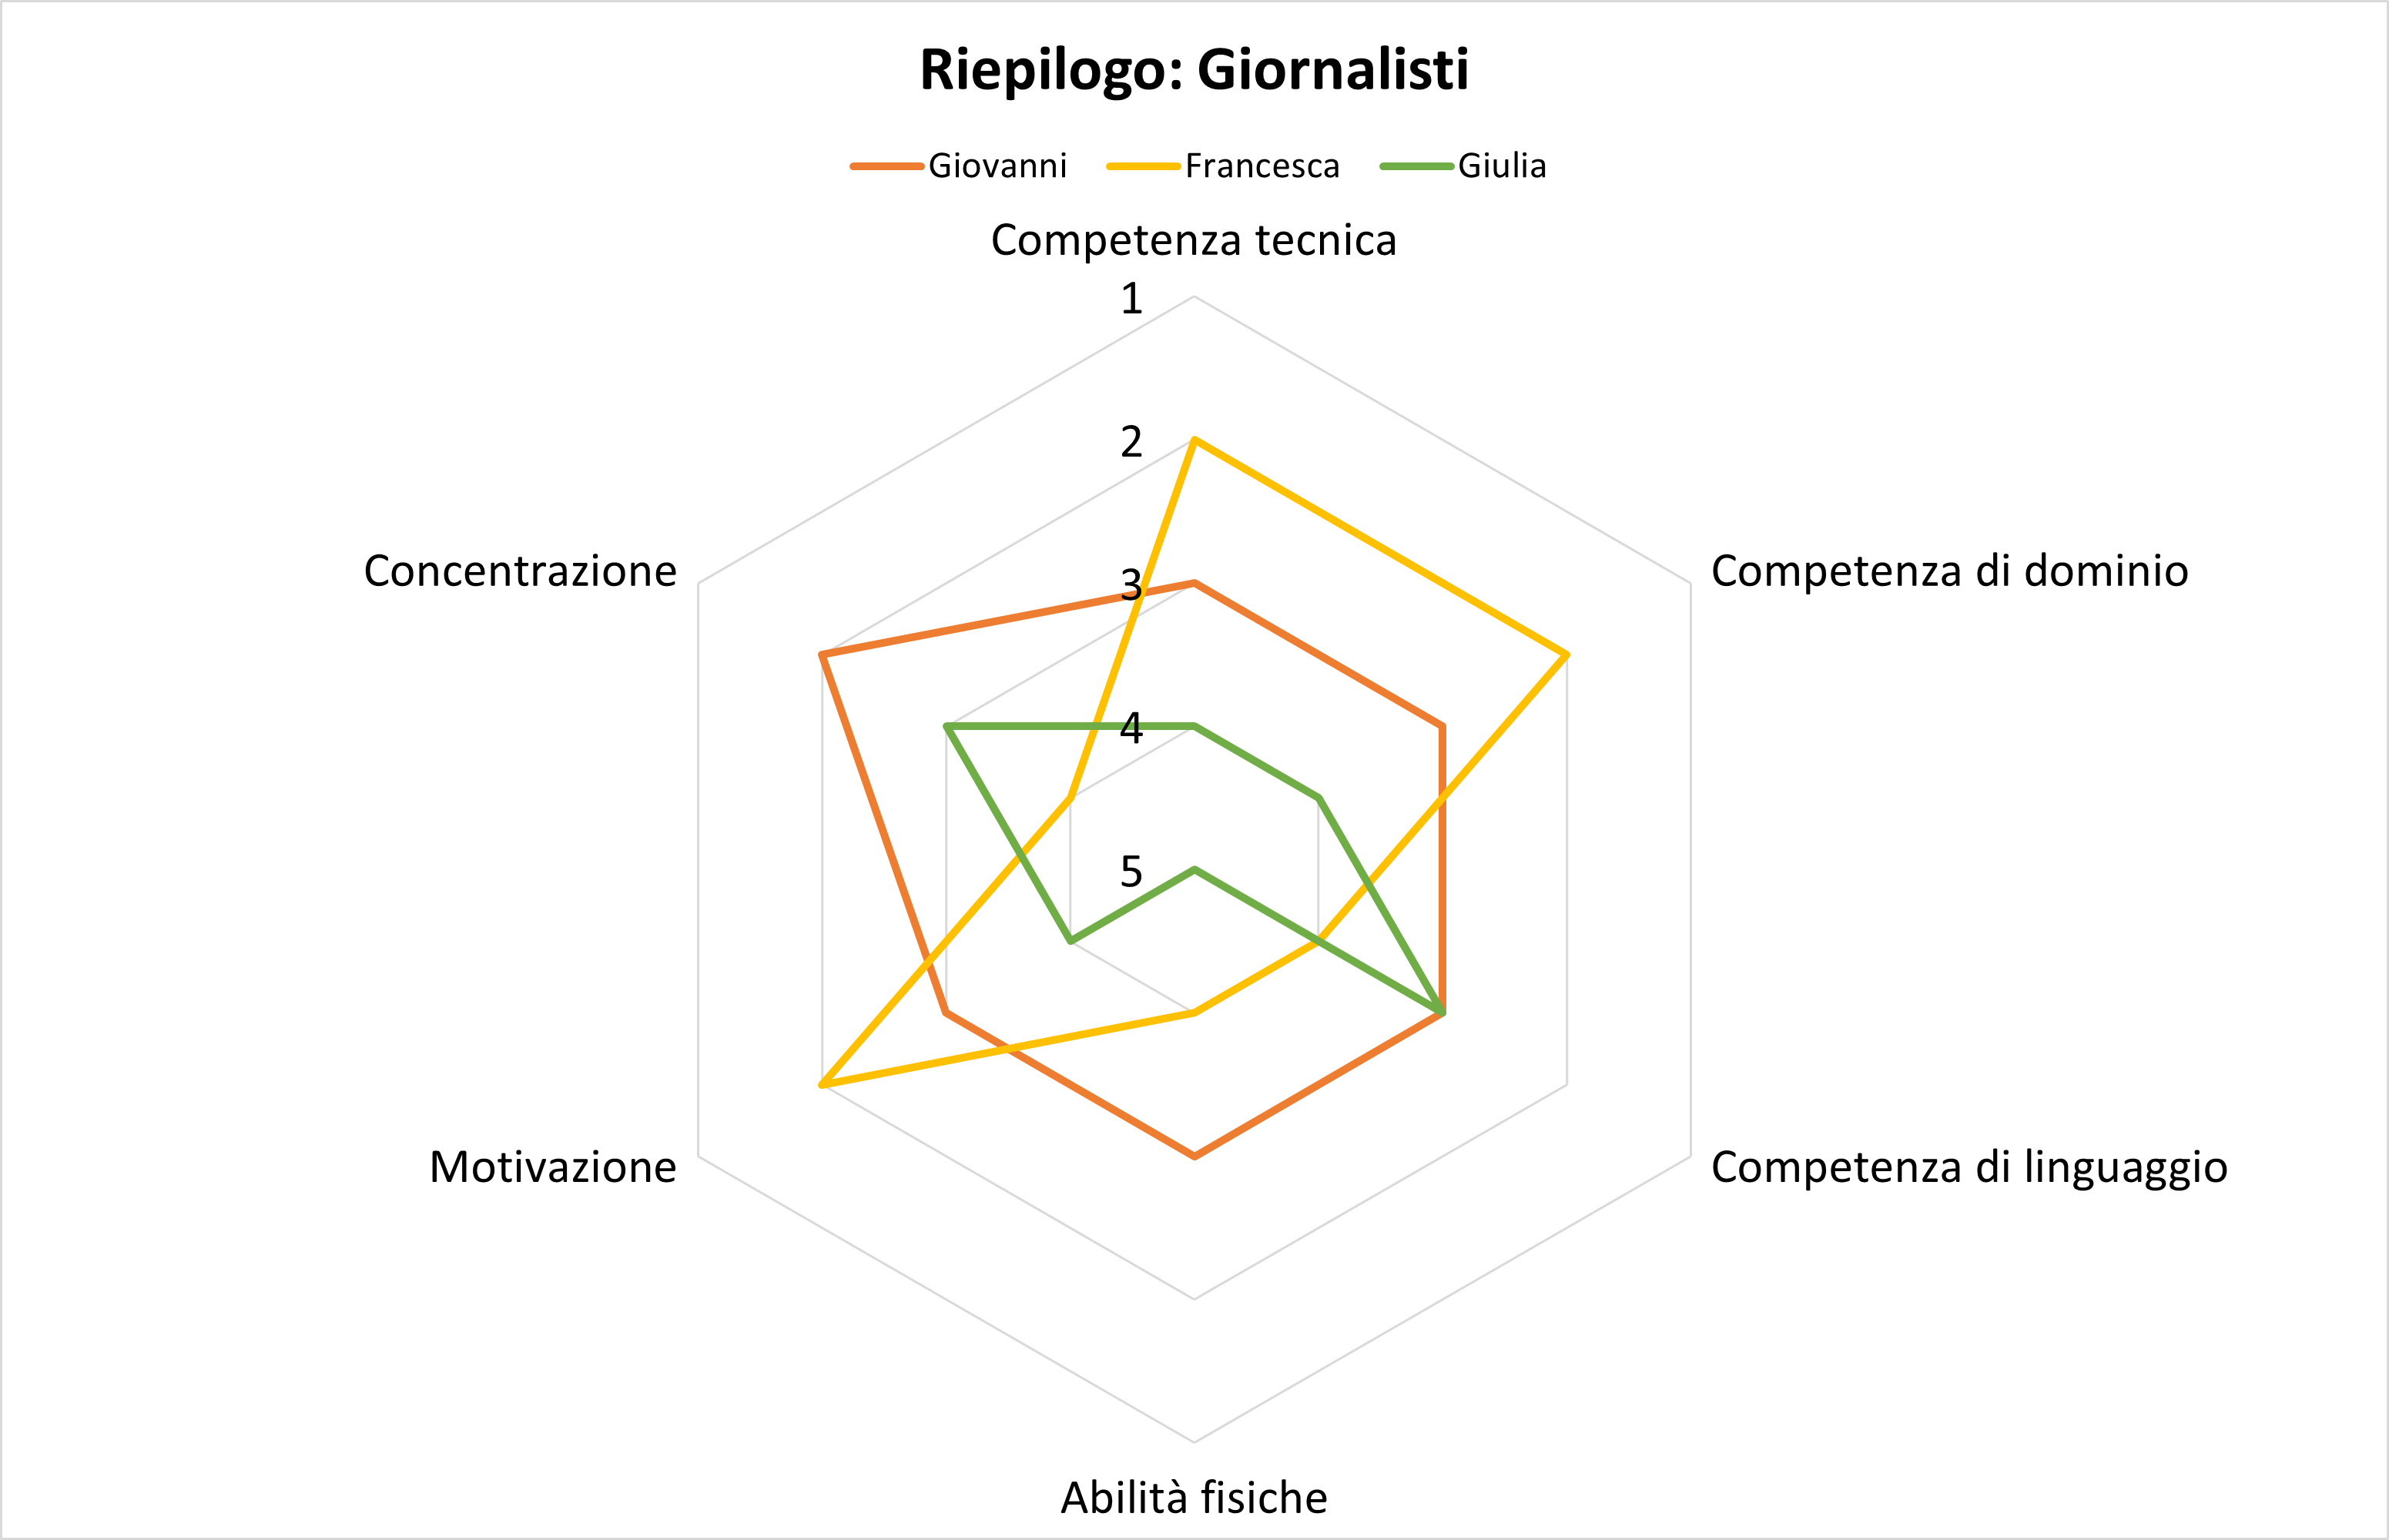
\includegraphics[width=0.5\columnwidth]{assets/images/proposta-design/caos/riepilogo-giornalisti}
    \caption{Diagramma C\&A di riepilogo sui giornalisti.}
\end{figure}

\noindent
Dal grafico relativo al cittadino esperto e al blogger, al contrario, è emersa una scarsa abilità fisica e competenza di linguaggio, il che ci ha portato a prevedere varie funzionalità in direzione dell'accessibilità, quali la possibilità di ingrandire i caratteri o di espandere a schermo intero i grafici, e un registro familiare per le etichette e le spiegazioni.
\begin{figure}[H]
    \centering
    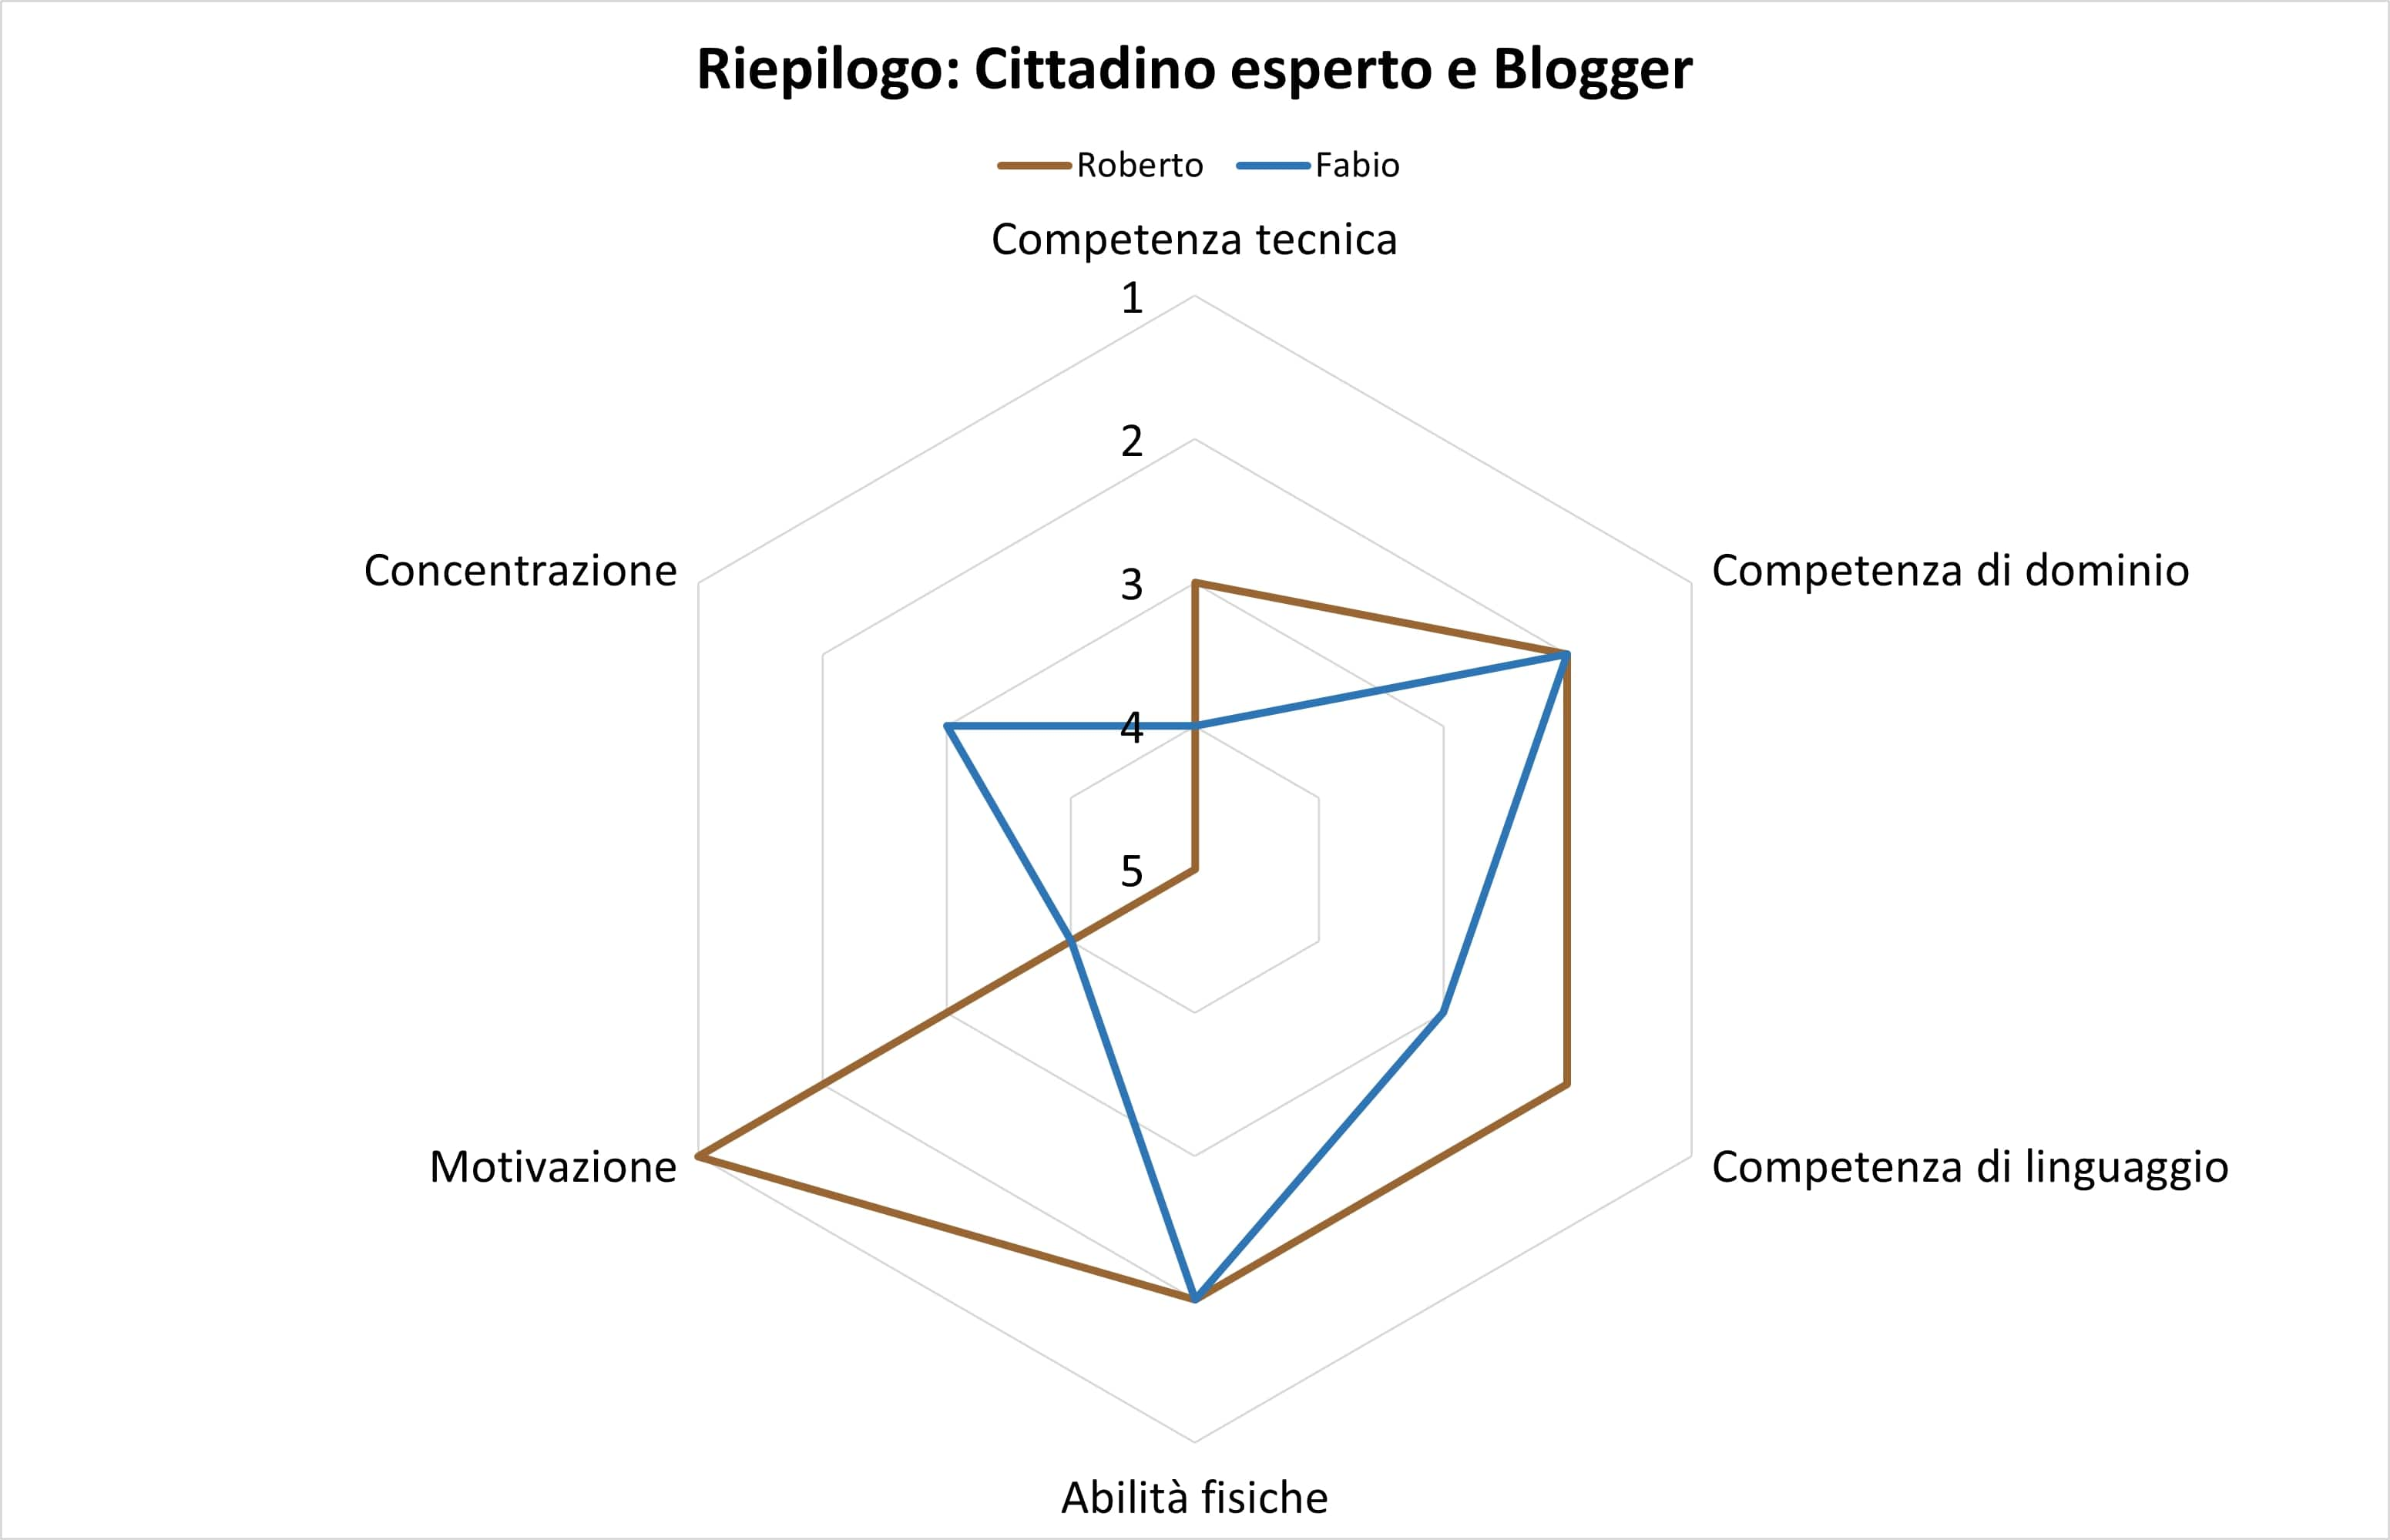
\includegraphics[width=0.5\columnwidth]{assets/images/proposta-design/caos/riepilogo-cittadini-altro}
    \caption{Diagramma C\&A di riepilogo sul blogger e il cittadino esperto.}
\end{figure}

\noindent
\subsubsection{Scenari a partire dagli attori}
\label{sss:scenari-a-partire-da-attori}
In seguito alla individuazione degli attori, il modello CAO=S prevede la definizione delle persona e degli scenari, per poi integrarli.
Abbiamo deciso di fare riferimento a quelli precedentemente elaborati nel capitolo \hyperref[c:studio-fattibilita]{3 Studio di Fattibilità}.
In particolare, per un'integrazione quanto più significativa, abbiamo rifinito alcuni aspetti marginali degli scenari, così da poter esaltare le peculiarità delle nostre persona mediante le attitudini e i comportamenti che hanno presentato nel realizzarli.\\
Gli scenari definiti in \ref{s:scenari} sono:
\begin{itemize}
    \item Scenario 1: Analisi dei dati quotidiani sull'andamento dell'epidemia Covid-19 in Italia;
    \item Scenario 2: Analisi dei dati quotidiani sull'andamento dell'epidemia Covid-19 in Emilia Romagna;
    \item Scenario 3: Analisi sull'andamento del tasso di letalità e sulla distribuzione dei numeri dell'epidemia relativamente alle due settimane precedenti;
    \item Scenario 4: Confronto dell'andamento dell'epidemia nelle regioni Emilia Romagna, Veneto e Molise nelle precedenti due settimane;
    \item Scenario 5: Confronto dell'andamento dell'epidemia in Italia nel mese corrente rispetto ai due mesi precedenti.
\end{itemize}
Le persona caratterizzate in \ref{s:persona} sono:
\begin{itemize}
    \item Giornalista testata nazionale: Giovanni;
    \item Giornalista testata locale: Francesca;
    \item Giornalista di agenzia di stampa: Giulia;
    \item Blogger: Roberto;
    \item Cittadino esperto: Fabio;
    \item Utente che consulta dashboard da dispositivo mobile: Christian.
\end{itemize}
\noindent
\paragraph{L'analisi quotidiana (scenario 1 svolto da Giulia)}\mbox{}\\
Giulia è una donna di 35 anni, laureata in Scienze Politiche all'Università di Milano.
Lavora per l'ANSA principalmente come ``fact-checker"; attualmente lavora da casa secondo la modalità di smart working che l'agenzia ha imposto a causa della pandemia.\\
Poco prima delle 17 accende il PC fornitole dall'agenzia e si collega alla dashboard del DPC.
Alle 17 e 4 minuti, la dashboard le notifica che i nuovi dati sono pronti e le suggerisce di aggiornare la pagina. Giulia esegue il suggerimento e la dashboard gli presenta i dati del giorno appena aggiornati: vede e trascrive nel documento Word precedentemente aperto i dati relativi al numero di nuovi positivi, di deceduti, di nuovi ingressi in terapia intensiva e al rapporto tra nuovi positivi e tamponi effettuati.
Oltre a questi dati, aggiunge all'articolo che sta scrivendo le immagini dei grafici che rappresentano l'andamento della pandemia.
Infine, per concludere la scrittura dell'articolo, legge le note della dashboard dove è riportato che la Liguria e la Valle d'Aosta hanno avuto problemi con la comunicazione dei dati e quindi integra nell'articolo anche queste informazioni.
\noindent
\paragraph{La situazione odierna della pandemia in Veneto (scenario 2 svolto da Francesca)}\mbox{}\\
Francesca è una donna di 36 anni di Mestre, laureatasi in Scienze della Comunicazione all'Università di Padova.\\
Lavora da sette anni presso la redazione del Gazzettino, in cui cerca di raccontare la propria regione e i suoi cittadini con passione, per fornire il proprio contributo diventato ancora più importante durante questa pandemia.\\
La sua giornata di lavoro sta per volgere al termine, tuttavia deve ancora redigere l'articolo quotidiano sull'andamento della pandemia nella sua regione, il Veneto.\\
In particolare, vuole comprendere se rispetto a ieri la situazione è migliorata, dato il quadro epidemiologico grave degli ultimi giorni. Si collega alla dashboard del DPC non appena nota che sono passate le ore 17.
Una volta aperta la dashboard, analizza i dati riportati per la regione: cerca il numero dei nuovi positivi, dei decessi, dei tamponi effettuati e quindi del tasso di positività. Può pertanto iniziare a redigere il suo articolo.\\
Francesca ha avuto una giornata piena di video-conferenze: in una ha anche intervistato il Sindaco di Padova che le ha rilasciato dichiarazioni circa le misure adottate dall'Università padovana per permettere la didattica in presenza; tra gli impegni della giornata, non ha avuto modo di informarsi circa eventuali ordinanze o dichiarazioni del Presidente della Regione.
Per colmare questa sua carenza informativa, interagisce con la sezione della dashboard che elenca i provvedimenti regionali: così facendo, viene a conoscenza di una nuova ordinanza emanata in mattinata, clicca sul link corrispondente e la legge. Quando ritorna sulla dashboard, la sua attenzione viene catturata da una notifica che la informa della correzione di alcuni dati.\\
Procede ad aggiornare il suo articolo e vi integrando le informazioni raccolte dall'intervista al Sindaco, nonché quelle relative al provvedimento letto.
\noindent
\paragraph{L'articolo di approfondimento (scenario 3 svolto da Giovanni)}\mbox{}\\
Giovanni è un uomo di 53 anni di Fiumicino, felicemente sposato da 24 anni e con due figlie.\\
Dopo aver completato gli studi presso l'Università La Sapienza di Roma e aver fatto esperienza in giornali locali, lavora ormai da 19 anni presso il Corriere della Sera, dove ricopre il ruolo di capo redattore.
In base al suo inquadramento, ha la responsabilità di scrivere articoli di approfondimento su temi di attualità: nel 2020, uno degli argomenti più accesi è la pandemia Covid-19, la quale, oltre a minacciare la sanità pubblica, sta stravolgendo gli assetti sociali, politici ed economici consolidatisi negli ultimi decenni.\\
Il 10 dicembre 2020 decide di redigere un articolo di analisi tramite cui fornire ai suoi lettori insight di valore circa il tasso di letalità e la distribuzione delle metriche epidemiologiche sui dati anagrafici, così da comunicare quali sono le categorie più a rischio.
Per acquisire le informazioni necessarie, si rivolge alla dashboard del DPC, divenuta negli ultimi mesi la sua fonte di riferimento, tantoché ha anche creato una configurazione dell'interfaccia ritagliata sui propri bisogni informativi.
Anzitutto recupera, con uno sguardo immediato, il tasso di letalità, per poi richiedere i dati delle principali metriche, in un formato che ne espliciti la distribuzione secondo l'età e il genere: dalla loro analisi, ravvisa una correlazione tra età e tasso di positività, secondo cui i soggetti più anziani sarebbero maggiormente esposti al contagio. 
\noindent
\paragraph{Il confronto fra il Veneto e la vicina Emilia-Romagna (scenario 4 svolto da Roberto)}\mbox{}\\
Il quadro epidemiologico del Veneto sta avendo uno sviluppo diametralmente opposto rispetto a quello dell'Emilia-Romagna.
Roberto, un uomo di 30 anni che di mestiere è un blogger e youtuber, si è interessato alla differenza dei quadri epidemiologici di cui sopra: in dettaglio, il suo interesse è nato dallo stimolo di un suo follower a tal proposito.\\
Pertanto, inizia le sue ricerche partendo dalla dashboard del DPC con la quale riesce a confrontare velocemente gli andamenti delle metriche epidemiologiche relative alle due regioni in oggetto: nota che in Veneto la situazione è molto peggiore che in Emilia-Romagna, in termini tanto di tasso di posività, quanto della media delle ospedalizzazioni giornaliere e dei decessi.
Roberto usa la dashboard anche per recuperare i vari provvedimenti emanati nelle due regioni e scopre che in Veneto sono state introdotte maggiori restrizioni solo nell'ultimo periodo. \\
Dopo essersi appuntato i dati visualizzati e aver fatto degli screenshot ai grafici, scrive il testo per il video che registrerà e pubblicherà il giorno seguente su questo tema.
\noindent
\paragraph{Comprensione profonda dei dati contro il sensazionalismo dei giornali (scenario 5 svolto da Fabio)}\mbox{}\\
Per i cittadini italiani, l'estate 2020 è stata un momento di tregua, covato ardentemente nei lunghi e difficili mesi precedenti, imperversati dalla pandemia Covid-19: le calde giornate estive hanno registrato numeri molto contenuti per le varie metriche epidemiologiche (nuovi positivi, ingressi nelle terapie intensive, deceduti…); inoltre, le misure restrittive imposte dal Governo per contrastare la diffusione del contagio sono state minime e mirate.
Questa nuova situazione sociale ed epidemiologica ha persuaso importanti fette della popolazione a lasciarsi andare in comportamenti rischiosi per il contagio, come assembramenti e scarso utilizzo di strumenti di protezione individuale.
Ed ecco che sul finire di agosto, il quadro epidemiologico positivo ha iniziato a cambiare peggiorare.\\
È il 2 settembre 2020 e Fabio, docente di Informatica all'università G. D'Annunzio di Pescara, è appena rientrato da un viaggio in compagnia di Claudia, sua moglie da ben 25 anni, e dei suoi figli.
Fabio non appartiene alla fetta di popolazione noncurante di cui sopra: anzi, anche durante le vacanze appena trascorse, ha indossato la mascherina in ogni ambiente chiuso o affollato, invitando anche la sua famiglia a fare altrettanto; inoltre, si informa quotidianamente sull'andamento delle metriche.
Da qualche giorno, gli è capitato di imbattersi più volte nella lettura di articoli giornalistici sul tema che, invece di riportare il peggioramento in atto del quadro sanitario, presentano toni ottimistici e superficiali, rasentando inesattezze e sottostime della realtà.
In particolare, da più fonti ha appurato che le ospedalizzazioni sono diminuite di un fattore di 10 rispetto a quelle registrate nel mese di maggio: questo dato gli sembra irrealistico, per cui si rivolge alla dashboard del DPC che solitamente consulta quando ha necessità di schiarirsi le idee.
Procede col richiedere il dato dei nuovi positivi alla data corrente (2 settembre '20) e la dashboard gli restituisce 1.326, valore che replica quasi esattamente i 1.327 nuovi positivi dell'8 maggio '20.
Focalizzandosi su queste due date confrontabili, richiede i dati dei ricoveri e trova 1.437 ricoverati con sintomi e 109 posti di terapia intensiva occupati del 2 settembre '20 rispetto ai 14.636 e 1.168 del 9 maggio '20.
Guardando esclusivamente questi valori assoluti, riscontra il rapporto di 1 a 10 tra i due periodi, come millantato dai giornali.
Tuttavia non è ancora convinto, per cui consulta siti istituzionali, alla ricerca di argomentazioni scientifiche circa l'analisi dei dati epidemiologici: scopre che le terapie intensive di un determinato giorno non sono espressione del numero dei nuovi positivi del giorno stesso, ma del cumulato dei positivi del mese precedente.
Ripete quindi la sua analisi sulla dashboard e trova i seguenti risultati: l'8 maggio '20 i 14.636 ricoverati e le 1.168 terapie intensive riflettevano quindi gli 81.599 positivi rilevati a partire dall'8 aprile '20, mentre il 2 settembre i 1.437 ricoverati e le 109 terapie intensive erano ``figli" dei 23.286 positivi rilevati a partire dal 3 agosto '20.
Alla luce di questa nuova consapevolezza, calcola che a maggio i ricoverati erano il 17,9\% dei positivi dei 30 giorni precedenti e le terapie intensive ne erano l'1,4\%, mentre a settembre il dato è rispettivamente 6,1\% e 0,4\%.
Il rapporto cambia completamente rispetto a quello rilevato usando i valori assoluti del singolo giorno: è circa un terzo, non un decimo.
Fabio, acquisita questa nuova informazione, la comunica sui social network su cui è iscritto, corredando il suo post con uno screenshot della parte della dashboard da cui ha tratto le sue conclusioni.
Ne parla quanto più in ogni occasione, in famiglia e con gli amici, al fine di aiutarli nella comprensione della reale situazione, certamente migliore di quella di maggio, ma non così rosea come si legge nei giornali, invitando sempre alla prevenzione del contagio.
\noindent
\paragraph{L'informazione quotidiana (nessuno scenario riconducibile, svolto da Christian)}\mbox{}\\
Christian è un uomo di 34 anni che lavora come fattorino per un'agenzia di logistica.
Ha un appartamento a Torino vicino a una fermata della metropolitana, che deve prendere necessariamente ogni giorno, per raggiungere la propria sede di lavoro.\\
A pranzo, quando è in pausa, è abituato ad informarsi sull'andamento della pandemia, nella consapevolezza che le restrizioni degli spostamenti e le chiusure dei negozi imposte per prevenirla possono aumentare gli acquisti on-line e quindi intensificare anche il suo lavoro di fattorino.
Leggendo un articolo su uno dei suoi siti abituali, viene a conoscenza di una dashboard sul Covid-19, utilizzata dai giornalisti.\\
Purtroppo però, accedendovi, scopre che non è fruibile per dispositivi mobili come il suo smartphone e quindi abbandona la pagina e torna a leggere il suo articolo.
\noindent
\paragraph{Caricamento quotidiano dei dati (nessuno scenario riconducibile, svolto dall'amministratore di database e dashboard)}\mbox{}\\
L'amministratore della base di dati collegata alla dashboard inserisce quotidianamente un'istanza per ciascuno dei seguenti concetti: andamento dele metriche epidemiologiche con granularità giornaliera dall'inizio della pandemia a livello nazionale, regionale e provinciale e dati delle metriche epidemiologiche relative alla data corrente a livello nazionale, regionale e provinciale.\\
Per la creazione di questi dati non utilizza la dashboard, bensì l'interfaccia del DBMS che gestisce la base di dati in questione.